\section{Surpression pulmonaire et décompression}

\begin{frame}{Surpression pulmonaire}
  \begin{block}{Définition}
    Lésion des poumons due à une \textbf{dilatation excessive de l’air} contenu dans les alvéoles,
    en cas de \textbf{blocage de la respiration à la remontée}.
  \end{block}

  \begin{itemize}
    \item L’air dans les poumons suit la loi de Mariotte.
    \item Si la remontée se fait \textbf{poumons fermés}, l’air ne peut pas s’échapper.
    \item Risque : \textbf{déchirure des alvéoles} et des vaisseaux sanguins.
    \item Accident de plongée \alert{le plus grave}.
  \end{itemize}
\end{frame}

\begin{frame}{Exemple et zone dangereuse}
  \begin{itemize}
    \item Capacité pulmonaire moyenne : \textbf{5 L}.
    \item À 20 m : $P = 3$ bar. Si on bloque à 20 m et qu’on remonte :
          \[
            3 \times 5 = 1 \times V_{\text{surface}} \Rightarrow V_{\text{surface}} = 15 \text{ L}
          \]
    \item Impossible pour les poumons : lésion bien avant la surface.
  \end{itemize}

  \begin{block}{Zone la plus dangereuse}
    Entre \textbf{0 et 10 m} : la pression est divisée par 2 $\Rightarrow$ le volume d’air est multiplié par 2.
  \end{block}
\end{frame}

\begin{frame}{Prévention de la surpression pulmonaire}
  \begin{columns}[c]
    \begin{column}{0.55\textwidth}
      \begin{alertblock}{Danger majeur}
        Ne jamais bloquer sa respiration à la remontée.
      \end{alertblock}
      \begin{itemize}
        \item Remonter à une \textbf{vitesse maximale de 15 m/min}.
        \item \textbf{Expirer doucement} tout au long de la remontée.
        \item Ne jamais donner d’air à un \textbf{chasseur en apnée}.
      \end{itemize}
    \end{column}
    \begin{column}{0.45\textwidth}
      \centering
      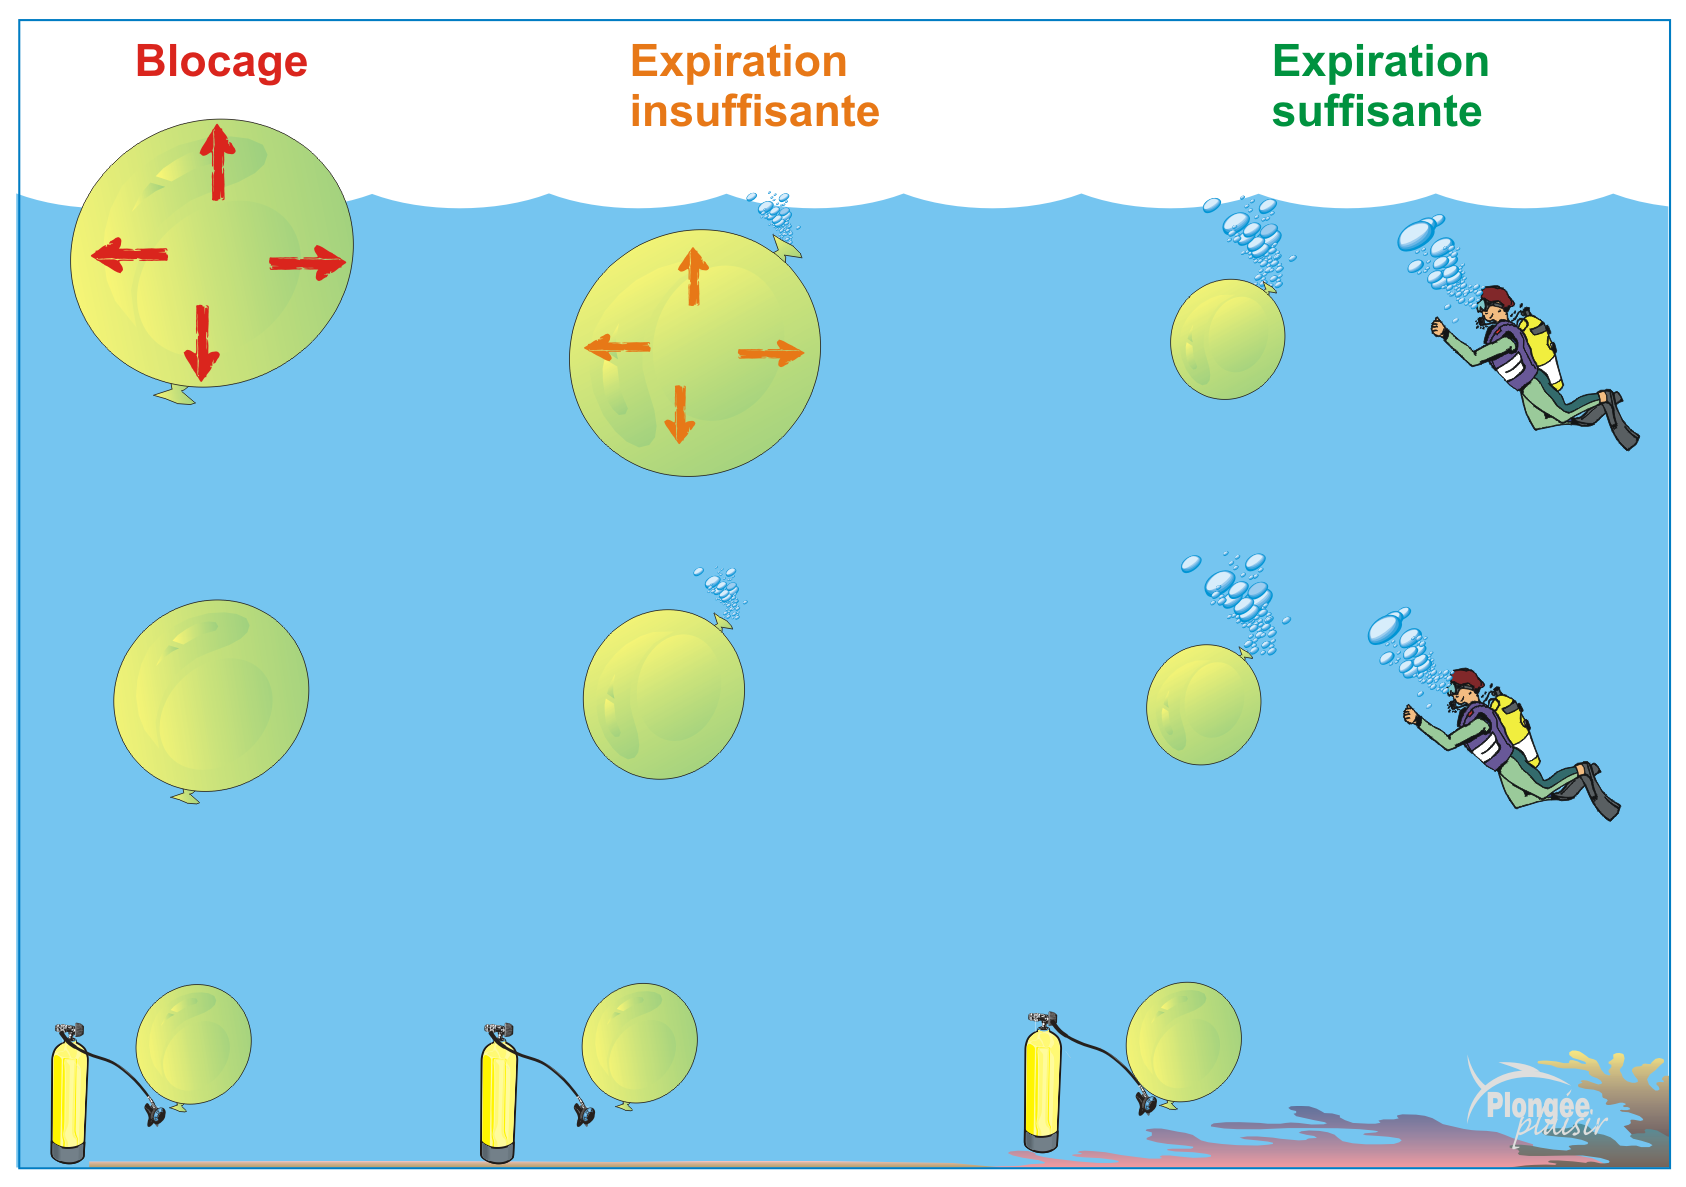
\includegraphics[height=0.6\textheight]{images/barotraumatisme-surpression-pulmonaire}
    \end{column}
    \end{columns}
\end{frame}

\begin{frame}{Accident de décompression}
  \begin{itemize}
    \item Air respiré : \textbf{~80 \% d’azote, ~20 \% d’oxygène}.
    \item L’azote se \textbf{dissout dans l’organisme} en fonction de la profondeur et du temps.
    \item Si la remontée est trop rapide ou les \textbf{paliers non respectés} :
          \begin{itemize}
            \item formation de \textbf{bulles d’azote} dans le sang et les tissus.
          \end{itemize}
  \end{itemize}
\end{frame}

\begin{frame}{Conséquences et prévention}
  \begin{block}{Conséquences possibles}
    \begin{itemize}
      \item Démangeaisons cutanées.
      \item Douleurs ostéo-articulaires.
      \item Atteintes neurologiques, cardiaques, pulmonaires, oreille interne…
    \end{itemize}
  \end{block}

  \begin{block}{Prévention}
    \begin{itemize}
      \item Rester dans la \textbf{courbe de sécurité}.
      \item Respecter la \textbf{vitesse de remontée maximale} 15 m/min et de préférence 10 m/min.
      \item Effectuer les \textbf{paliers obligatoires} et un palier de sécurité
            de \textbf{3 min à 3 m}.
      \item Éviter les efforts importants après la plongée.
      \item Ne pas plonger fatigué.
    \end{itemize}
  \end{block}
\end{frame}
